\section{Stabilität im Bodediagramm}

\fbox{\parbox{0.95\columnwidth}{
Es gilt, dass wenn der \textbf{offene} Regelkreis $H(s)$ nur Pole in der linken $s$-Halbebene hat (und höchstens zwei Pole 
im Ursprung bei $s = 0$), der \textbf{geschlossene} Regelkreis genau dann \textbf{asymptotisch stabil} ist, wenn $H(\jimg \omega)$
für die \textbf{Durchgangsfrequenz} $\omega_D$ bei der die Amplitude $20 \cdot \log_{10}(|H(\jimg \omega_D)|) = 0 \, \deci \bel$
ist, und eine Phase $> - \pi$ hat. \\
\textrightarrow\ Amplitudenrand und Phasenrand müssen $> 0$ sein, damit das System stabil ist!
}}


\subsection{Amplitudenrand und Phasenrand }

\begin{outline}
    \1 \textbf{Amplitudenrand (Verstärkungsreserve)}
        \2 Abstand des Amplitudengangs zur $0 \, \deci \bel$-Linie bei der Kreisfrequenz $\omega$, bei der die Phase 
        gleich $- \pi$ bzw. $- 180 \degree$ ist.
    \1 \textbf{Phasenrand (Phasenreserve)}
        \2 Abstand des Phasengangs zur $- \pi$-Linie bei der Kreisfrequenz $\omega$, bei der die Amplitude 
        gleich $0 \, \deci \bel$ ist.
\end{outline}


\subsection{Amplitudenrand und Phasenrand im Bodediagramm}

\begin{minipage}[c]{0.65\columnwidth}
    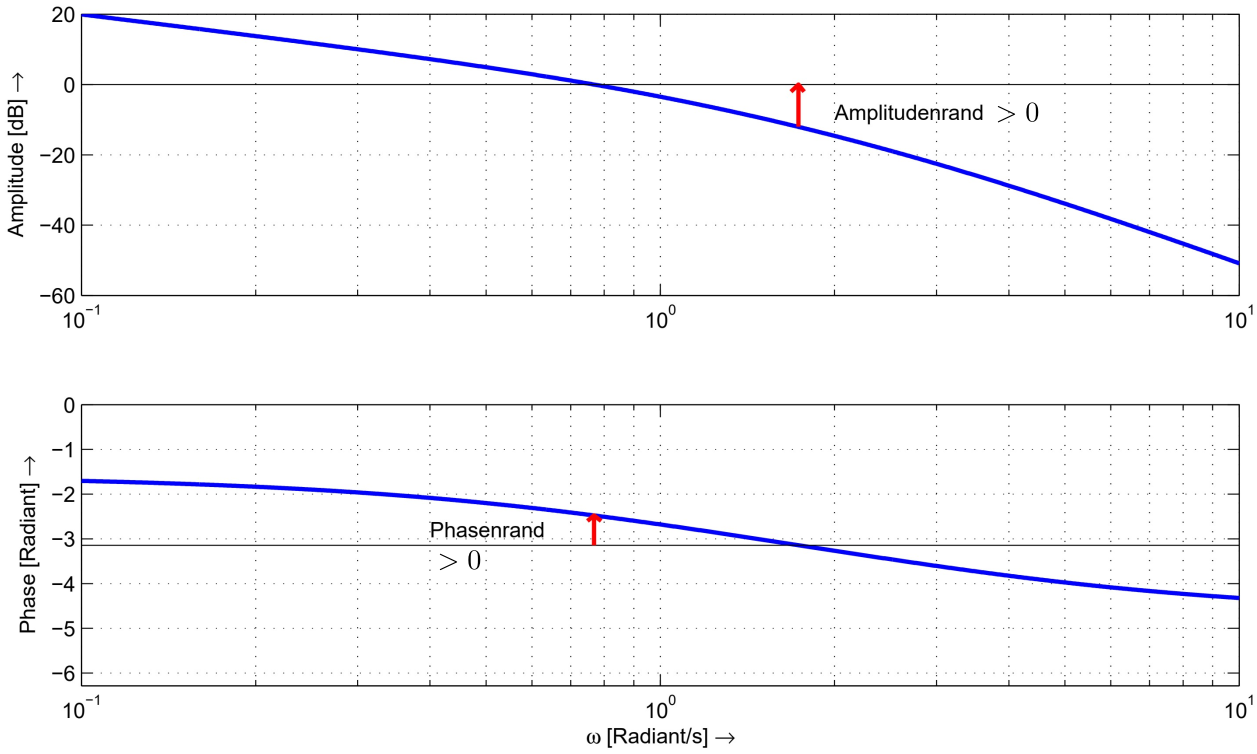
\includegraphics[width=\columnwidth]{images/bode_amplitudenrand_phasenrand.png}
\end{minipage}
\hfill
\begin{minipage}[c]{0.32\columnwidth}
    Das System ist \textbf{stabil}, da sowohl Amplitudenrand als auch Phasenrand $> 0$ sind.
\end{minipage}

